\chapter{Lost Lepton Background}
\label{chap:lostlep}

A second source of background comes from events where a genuine prompt lepton is produced
from the decay of a $W$ boson. While the tight lepton veto employed in the analysis 
aims to eliminate as many of these events as possible, a significant number still enter
the signal regions because the lepton gets ``lost''. This can happen for a number
of reasons, such as the lepton being outside of the acceptance window (i.e. it is too forward
 or the \pt is too small) or not being isolated, or the reconstruction algorithms
failing to identify the candidate as a lepton. 

Generally the energy of the lepton is still
accounted for (making ``lost'' a bit of a misnomer), so there is no fake \ptmiss from the lepton. 
However, there is real \ptmiss from the neutrino from the $W$ decay, and this is often enough
to allow the event to enter the signal region. The dominant production mechanisms for the lost
lepton background are \wjets and \ttbar production, but there are also smaller contributions
from rarer processes such as single top, $\ttbar W$, $\ttbar Z$, $\ttbar H$, and $tt\bar{t}\bar{t}$.

The lost lepton background is estimated in a data-driven way using a control sample of events
where there \emph{is} a reconstructed lepton. Section~\ref{sec:llep_pred} describes how this
is done in each $(\Ht, \Nj, \Nb)$ topological region, Sec.~\ref{sec:llep_mt2} explains the method
for extrapolating along the \mttwo dimension, and Sec.~\ref{sec:llep_syst} lists the systematic
uncertainties assessed on the final estimate.

\section{Prediction from single lepton control regions}
\label{sec:llep_pred}

\begin{figure}[htbp]
  \begin{center}
    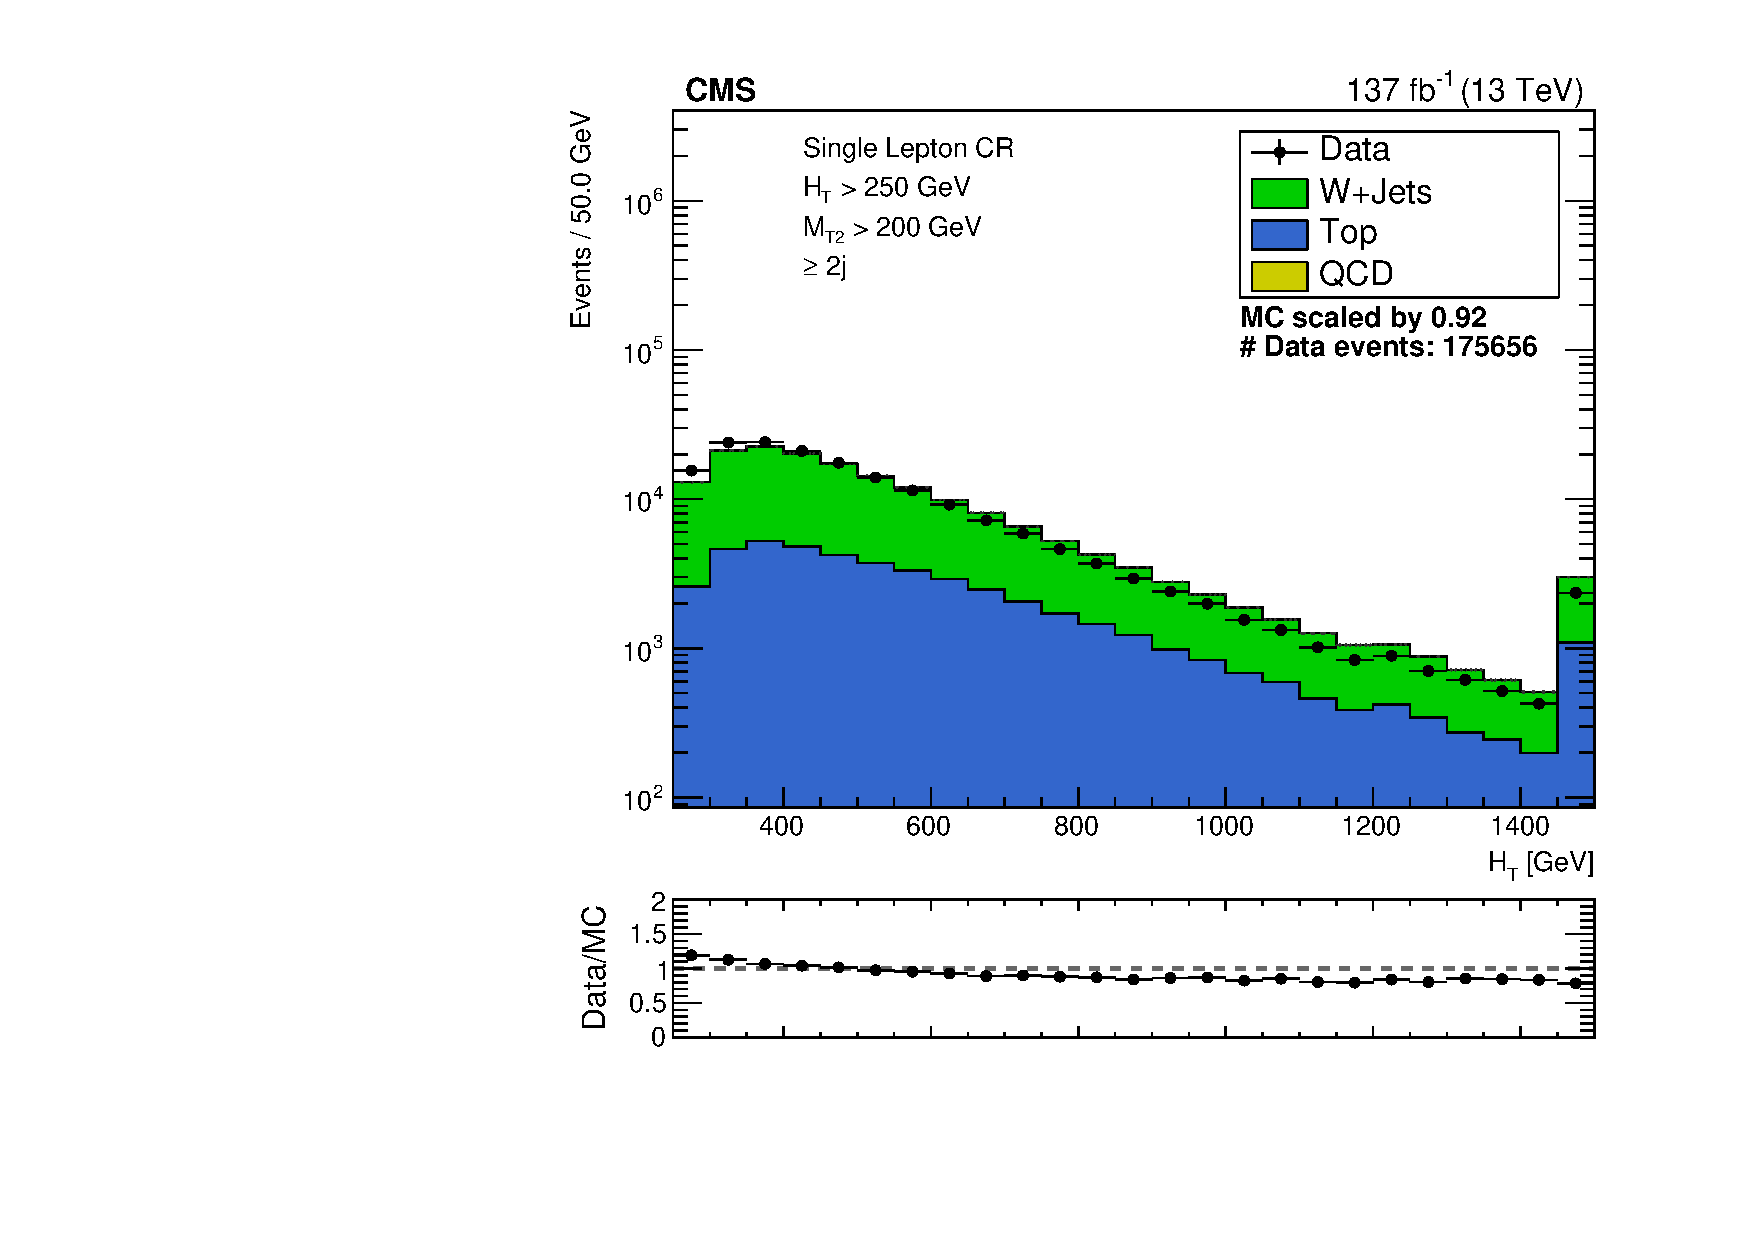
\includegraphics[width=0.47\textwidth]{figs/llep/crslbase_ht.pdf}
    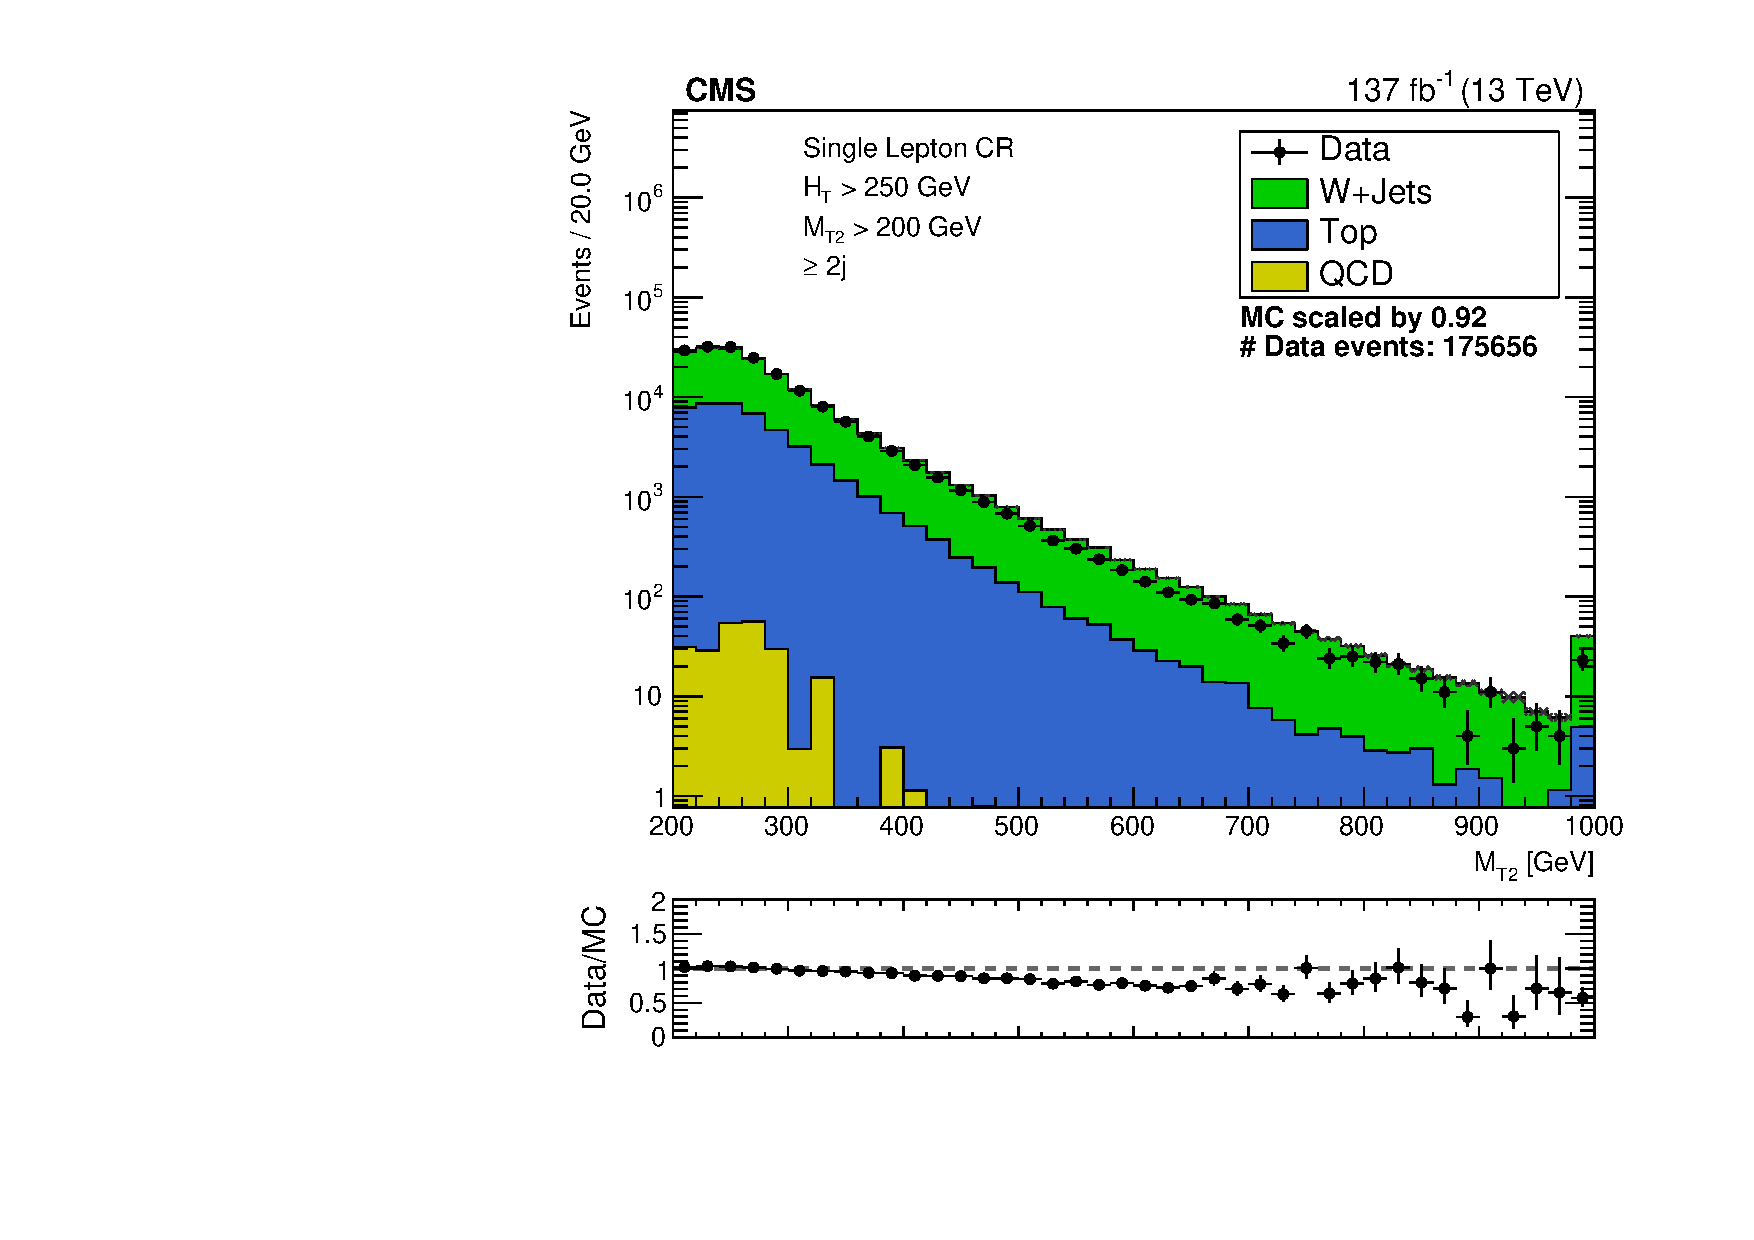
\includegraphics[width=0.47\textwidth]{figs/llep/crslbase_mt2.pdf} \\
    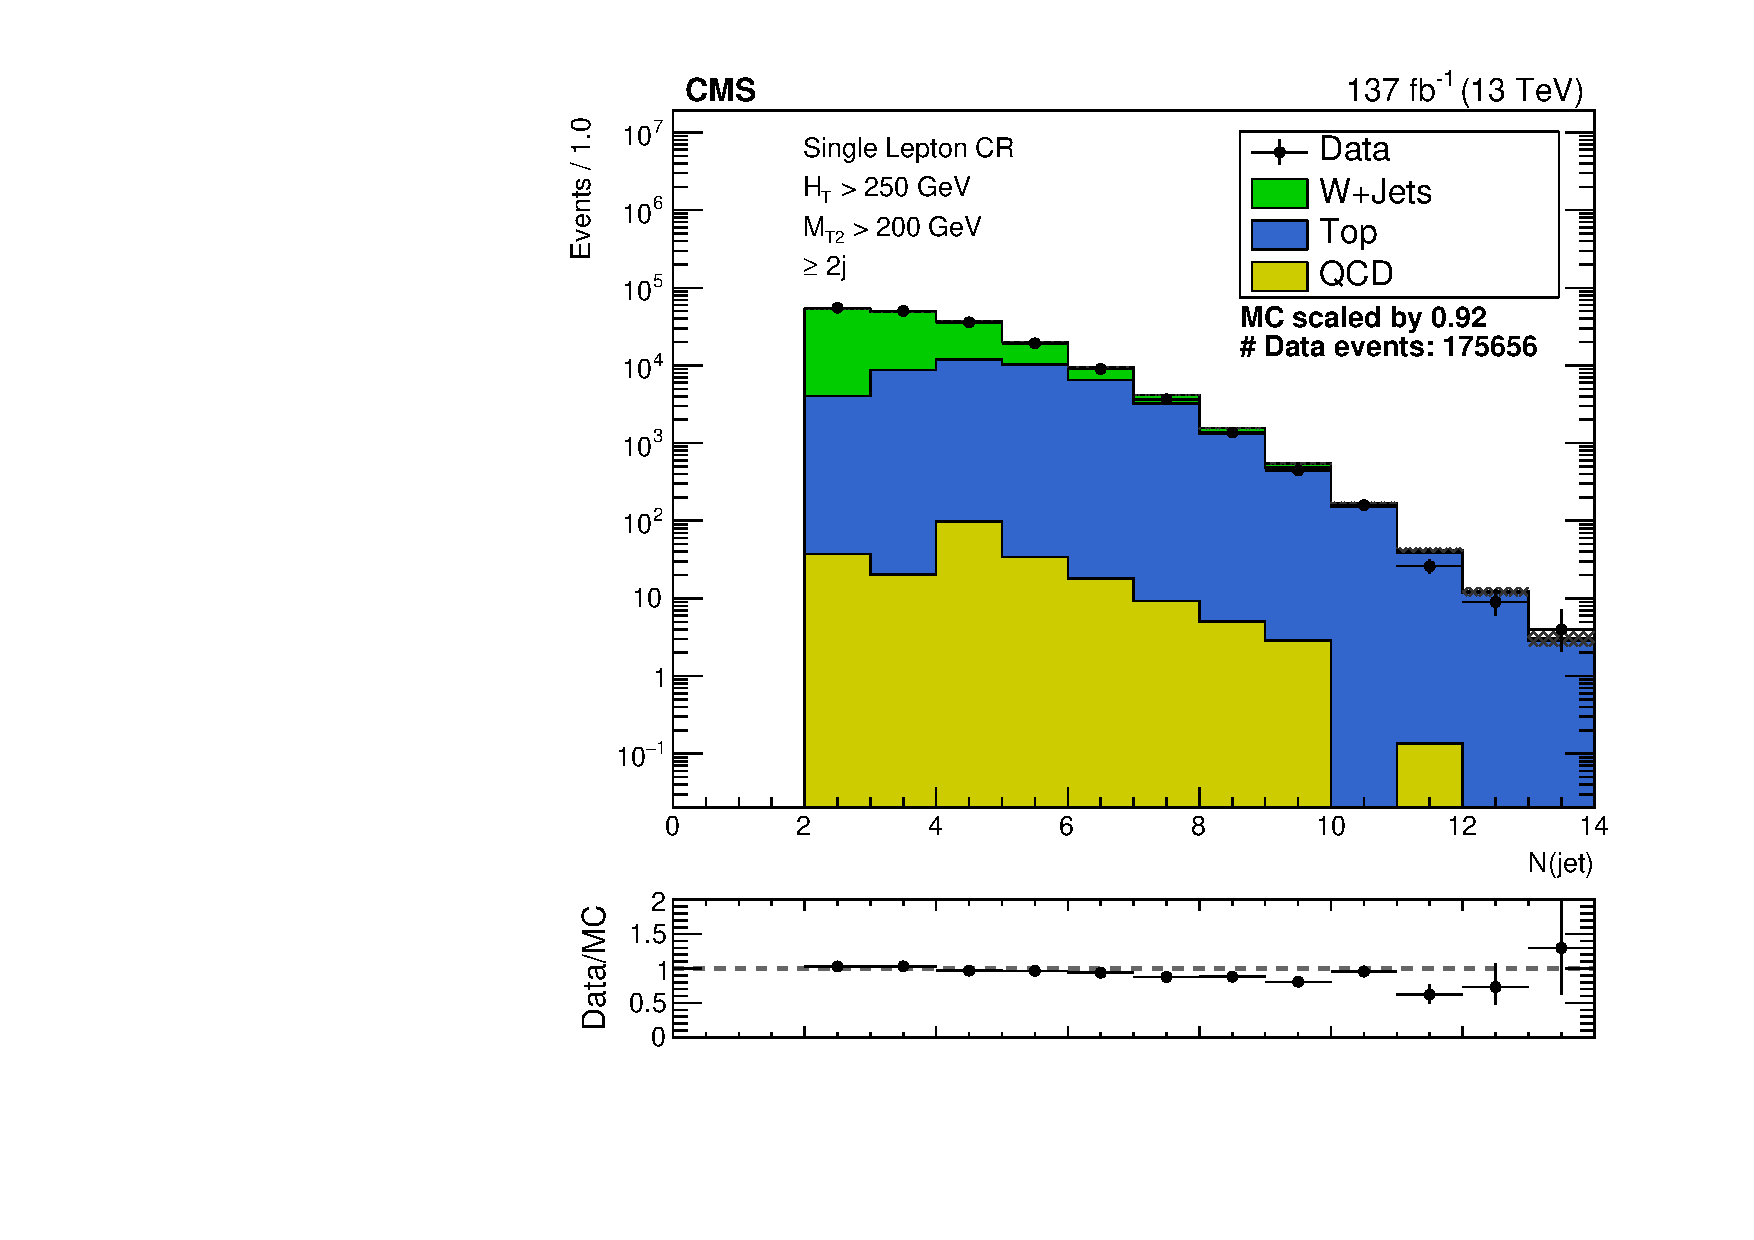
\includegraphics[width=0.47\textwidth]{figs/llep/crslbase_nJet30.pdf}
    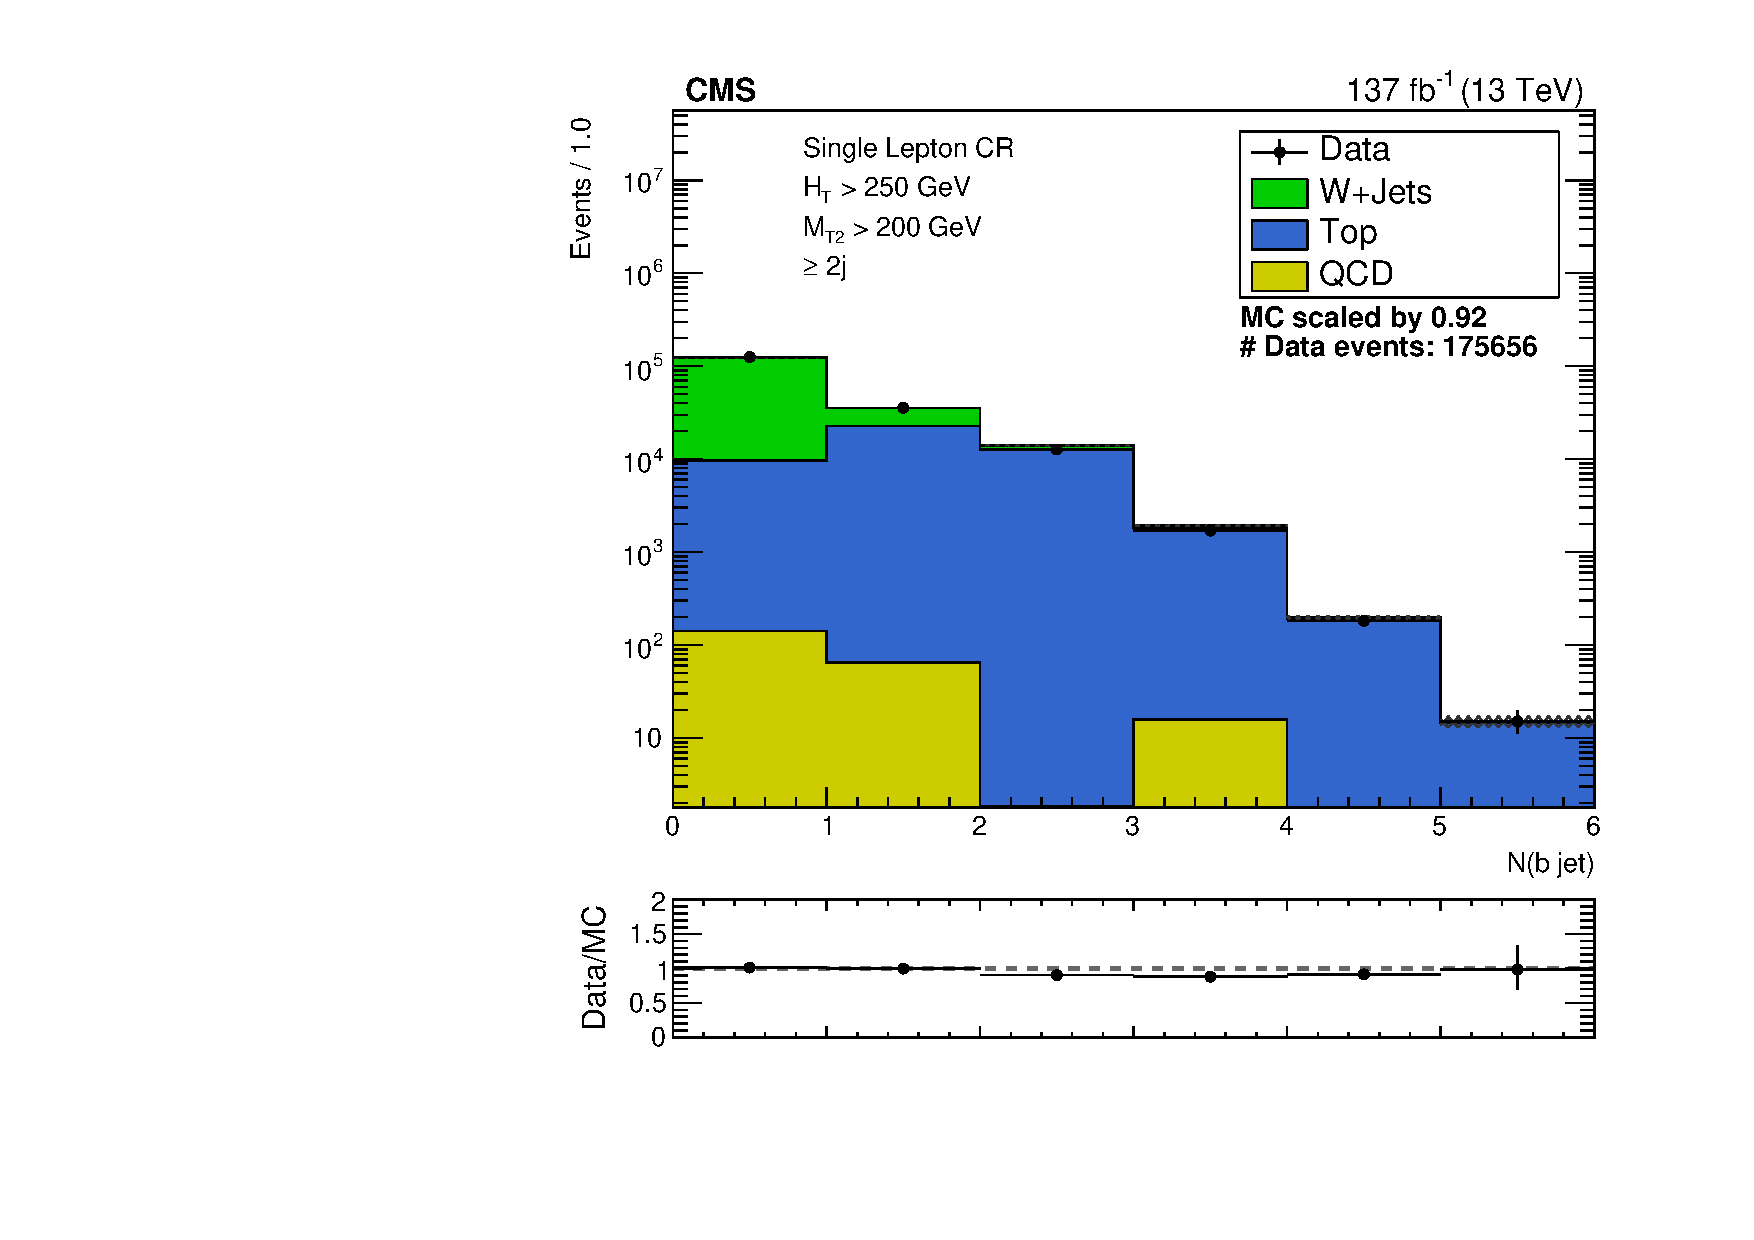
\includegraphics[width=0.47\textwidth]{figs/llep/crslbase_nBJet20.pdf} \\
    \caption{Data vs.\ MC comparisons in the baseline single lepton control region, for $\Nj\geq2$.
      From left to right, top to bottom, the variables
      plotted are \Ht, \mttwo, \Nj, and \Nb.
            }
    \label{fig:llep_crplots}
  \end{center}
\end{figure}

\subsection{$\ttbar+\text{heavy flavor}$ modeling}

\subsection{Signal contamination}

\section{\texorpdfstring{\mttwo}{MT2} extrapolation}
\label{sec:llep_mt2}

\section{Systematic uncertainties}
\label{sec:llep_syst}
